\documentclass[12pt]{article}

\usepackage[CJKnumber]{xeCJK}
\setCJKmainfont{Iansui 094}
\usepackage[a4paper, margin=1.5cm]{geometry}
\usepackage{graphicx}
\usepackage{amsmath, amsfonts, amssymb}

\newcommand{\testtitle}[1]{ \begin{center}{\large\bf #1}\end{center} }

\begin{document}

\testtitle{怪怪數學題目}

\section{前言}

數列與級數是個適合發揮創意的題目類型。有時候把東西搬來搬去就做完了(?

\section{暖身題}

\begin{enumerate}
	\item 一個 $x$-連通塊代表將 $x$ 個小正方形以邊相接連成一塊的形狀,例如俄羅斯方塊就是 4-連通塊。已知 7-連通塊有 108 種,求能不能把這 108 個 7-連通塊排成一個 $7 \times 108$ 的大矩形?證明可以或不行。
		\vspace{10mm}
	\item 下面圖形每條直線皆等長,所有角度皆為 $45^\circ$ 的倍數,請將此形狀分為五塊全等的區域。作答時間:直到放棄,或是發現他其實很簡單。
		\begin{center} 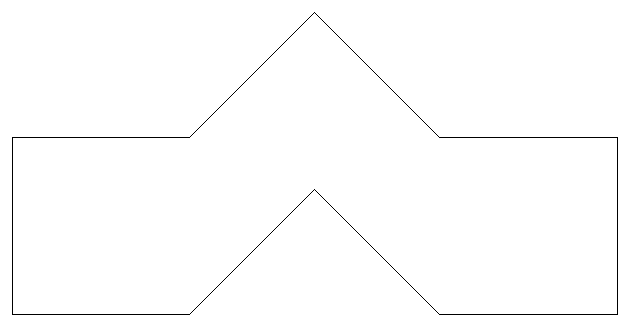
\includegraphics[width=0.4\textwidth]{a.pdf} \end{center}
		\vspace{10mm}
	\item 令 $S_n = \sum _ {i = 1} ^{n} {a_i}$ ,已知 $S_n = n^2 + 3n + 1$ ,求 $a_n$ 的一般式。
		\vspace{10mm}
	\item 令 $a_n$ 為第 $n$ 圖的周長,已知 $a_1 = 3$ ,求 $\sum _{i=1} ^{\infty} \frac{1}{a_i}$ 。
		\begin{center} 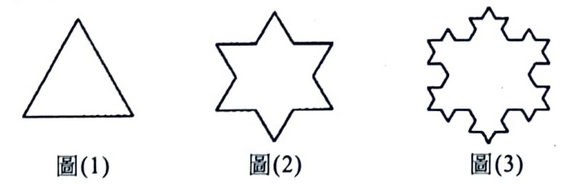
\includegraphics[width=0.4\textwidth]{EE0808.png} \end{center}
		\vspace{10mm}
\end{enumerate}

\section{一些名詞雜燴}

\begin{enumerate}
	\item 公比:不能為 $0$ ,不然後面的比會沒辦法定義。
	\item $\sum _ {i = a} ^ {b} f(i)$ :把 $f(a), f(a+1), f(a+2), \cdots, f(b)$ 加起來。
	\item $\prod _ {i = a} ^ {b} f(i)$ :把 $f(a), f(a+1), f(a+2), \cdots, f(b)$ 乘起來。
	\item 曲率半徑:假裝一段弧線是某個圓的一部分,求那個圓的半徑。
\end{enumerate}

\pagebreak

\section{數列與級數}

\subsection{通靈消消消}

\begin{enumerate}
	\item 求 $\sqrt[256]{(2+1)(2^2+1)(2^4+1)\cdots(2^{256}+1)+1}$ 。
		\vspace{10mm}
	\item 已知 $k \ne 1$ ,求 $\sum _{i=1} ^ {n} k^i$ 。
		\vspace{10mm}
	\item 已知 $k \ne 1$ ,求 $\sum _{i=1} ^ {n} i \cdot k^i$ 。
		\vspace{30mm}
	\item 如圖,已知每一列數字為上一列相鄰兩數的和,求圖中最下面的數字(以 $n$ 表示)。
		\begin{center} 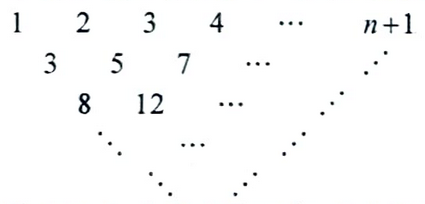
\includegraphics[width=0.4\textwidth]{CS1718.png} \end{center}
		\vspace{10mm}
\end{enumerate}

\subsection{進階的等比數列}

\begin{enumerate}
	\item 已知 $a_1 = 2, a_n = 2a_{n-1} (\forall n \ge 2)$ ,求 $a_n$ 一般式。
		\vspace{10mm}
	\item 已知 $a_1 = 5, a_2 = 7, a_n = 3a_{n-1} - 2a_{n-2} (\forall n \ge 3)$ ,求 $a_n$ 一般式。
		\vspace{30mm}
	\item 已知 $a_1 = 1, a_2 = 4, \sqrt{a_n a_{n-2}} = 2\sqrt{a_{n-1}a_{n-2}} + p a_{n-1}$ ,求 $a_n$ 一般式。
		\vspace{30mm}
\end{enumerate}

\pagebreak

\subsection{奇怪的作法}

\begin{enumerate}
	\item 已知 $a_1 = \sqrt{12}, a_n = \sqrt{12 + a_{n-1}}$ ,已知 $n$ 接近無限大時 $a_n$ 會接近某一數值 $x = \lim _ {n \rightarrow \infty} a_n$ ,求 $x$ 。
		\vspace{30mm}
	\item 已知 $F_1 = F_2 = 1, F_n = F_{n-1} + F_{n-2} (\forall n \ge 3)$ ,求 $\lim _ {n \rightarrow \infty} \frac{F_n}{F_{n-1}}$ ( $n$ 接近無限大時 $\frac{F_n}{F_{n-1}}$ 是多少)。
		\vspace{30mm}
\end{enumerate}

\subsection{勇氣很重要}

\begin{enumerate}
	\item 求 $\sum _ {x = 0} ^ {\infty} \frac{\cos 60x ^ \circ}{2^x}$ 。
		\vspace{10mm}
\end{enumerate}

\end{document}
